\documentclass[tikz,border=6pt]{standalone}
\usetikzlibrary{decorations.pathreplacing, arrows.meta}

\begin{document}
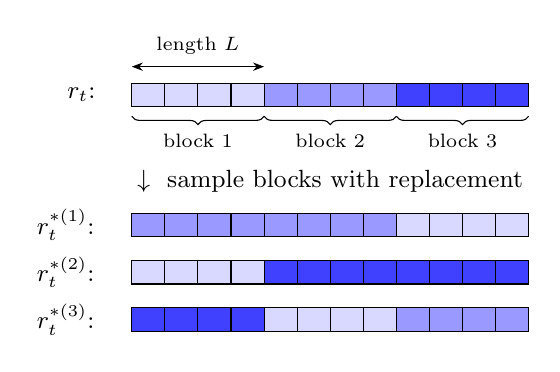
\begin{tikzpicture}[
    cell/.style={draw, minimum width=0.42cm, minimum height=0.3cm, inner sep=0pt},
    lab/.style={font=\small},
    blab/.style={font=\scriptsize},
    note/.style={font=\tiny, text=black!55},
  ]

  % r_t row: 3 blocks of 4 cells each, increasing blue intensity
  \node[lab] at (-0.85, 0) {$r_t$:};
  \foreach \i in {0,...,3}
  \node[cell, fill=blue!15] at (\i*0.42, 0) {};
  \foreach \i in {4,...,7}
  \node[cell, fill=blue!40] at (\i*0.42, 0) {};
  \foreach \i in {8,...,11}
  \node[cell, fill=blue!75] at (\i*0.42, 0) {};

  % L: block length, illustrated directly above block 1
  \draw[{Stealth[length=4pt]}-{Stealth[length=4pt]}]
  (-0.21, 0.36) -- (1.47, 0.36) node[midway, above=1pt, blab] {length $L$};

  % block labels underneath, via braces
  \draw[decorate, decoration={brace, amplitude=3pt, mirror}]
  (-0.21, -0.27) -- (1.47, -0.27) node[midway, below=3pt, blab] {block 1};
  \draw[decorate, decoration={brace, amplitude=3pt, mirror}]
  (1.47, -0.27) -- (3.15, -0.27) node[midway, below=3pt, blab] {block 2};
  \draw[decorate, decoration={brace, amplitude=3pt, mirror}]
  (3.15, -0.27) -- (4.83, -0.27) node[midway, below=3pt, blab] {block 3};

  % arrow + caption
  \node[lab] at (2.31, -1.1) {$\downarrow$ \ sample blocks with replacement};

  % three independent resamples -- some blocks repeat, some never show up
  \node[lab] at (-1.05, -1.65) {$r_t^{*(1)}$:};
  \foreach \i in {0,...,3}
  \node[cell, fill=blue!40] at (\i*0.42, -1.65) {};
  \foreach \i in {4,...,7}
  \node[cell, fill=blue!40] at (\i*0.42, -1.65) {};
  \foreach \i in {8,...,11}
  \node[cell, fill=blue!15] at (\i*0.42, -1.65) {};
  % \node[note, anchor=west] at (5.15, -1.65) {block 3 never drawn};

  \node[lab] at (-1.05, -2.25) {$r_t^{*(2)}$:};
  \foreach \i in {0,...,3}
  \node[cell, fill=blue!15] at (\i*0.42, -2.25) {};
  \foreach \i in {4,...,7}
  \node[cell, fill=blue!75] at (\i*0.42, -2.25) {};
  \foreach \i in {8,...,11}
  \node[cell, fill=blue!75] at (\i*0.42, -2.25) {};
  % \node[note, anchor=west] at (5.15, -2.25) {block 2 never drawn};

  \node[lab] at (-1.05, -2.85) {$r_t^{*(3)}$:};
  \foreach \i in {0,...,3}
  \node[cell, fill=blue!75] at (\i*0.42, -2.85) {};
  \foreach \i in {4,...,7}
  \node[cell, fill=blue!15] at (\i*0.42, -2.85) {};
  \foreach \i in {8,...,11}
  \node[cell, fill=blue!40] at (\i*0.42, -2.85) {};
  % \node[note, anchor=west] at (5.15, -2.85) {each block once};

\end{tikzpicture}
\end{document}
